\centerline{\Huge \bf  Домашняя работа}
\centerline{\Huge \bf Разрезания начало}

\begin{flushright}
    \scriptsize{Чем БОЛЬШЕ разрезаний, тем БОЛЬШЕ баллов!}
\end{flushright}


\problem{1!} 
Разделите фигуру на три равные части так, чтобы линия разреза шла по сторонам квадратов.
\begin{figure}[h]
        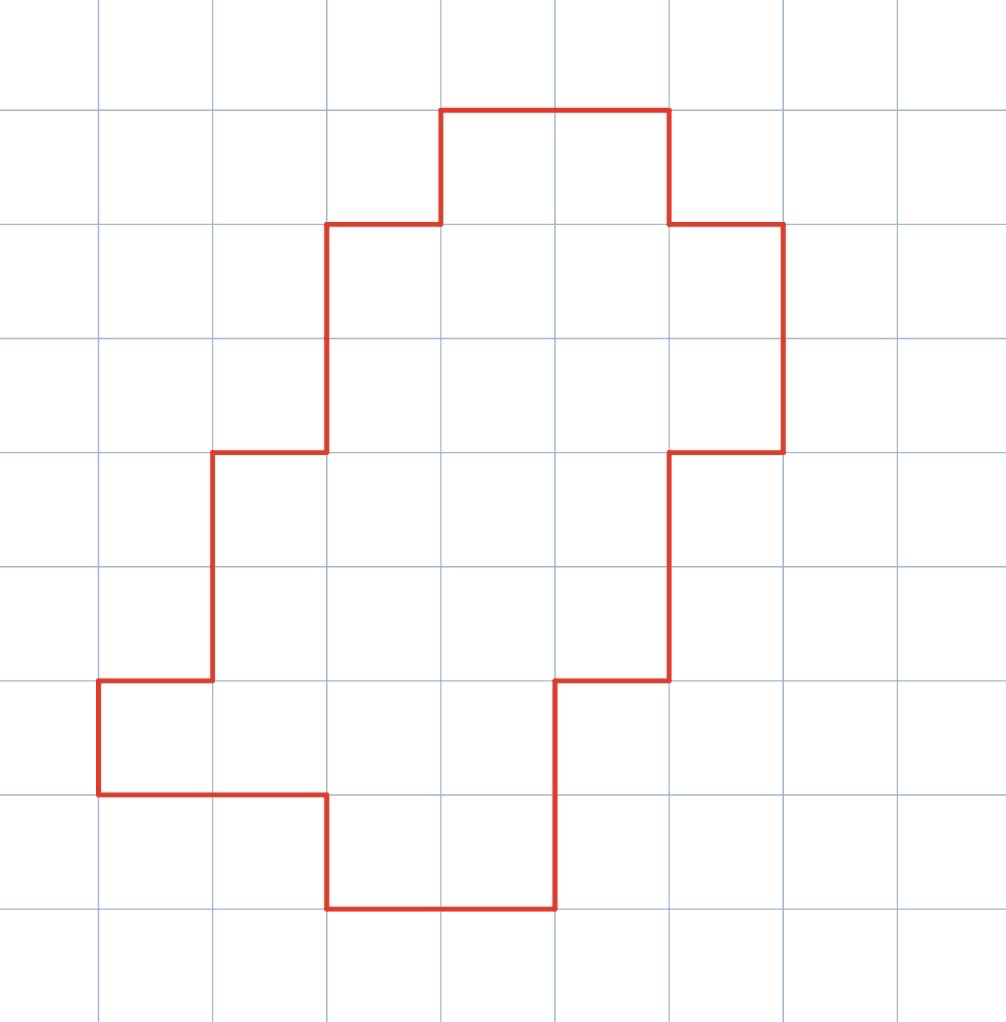
\includegraphics[width=0.2\linewidth]{ЭлМШ 2023-2024/VIII блок/Шиншиллы/HW_Cutting_1.png}
\end{figure}

\problem{2!}
Разрежьте фигуру на пять равных частей по линиям сетки, причем в каждой из частей должна быть одна точка.
\begin{figure}[h]
        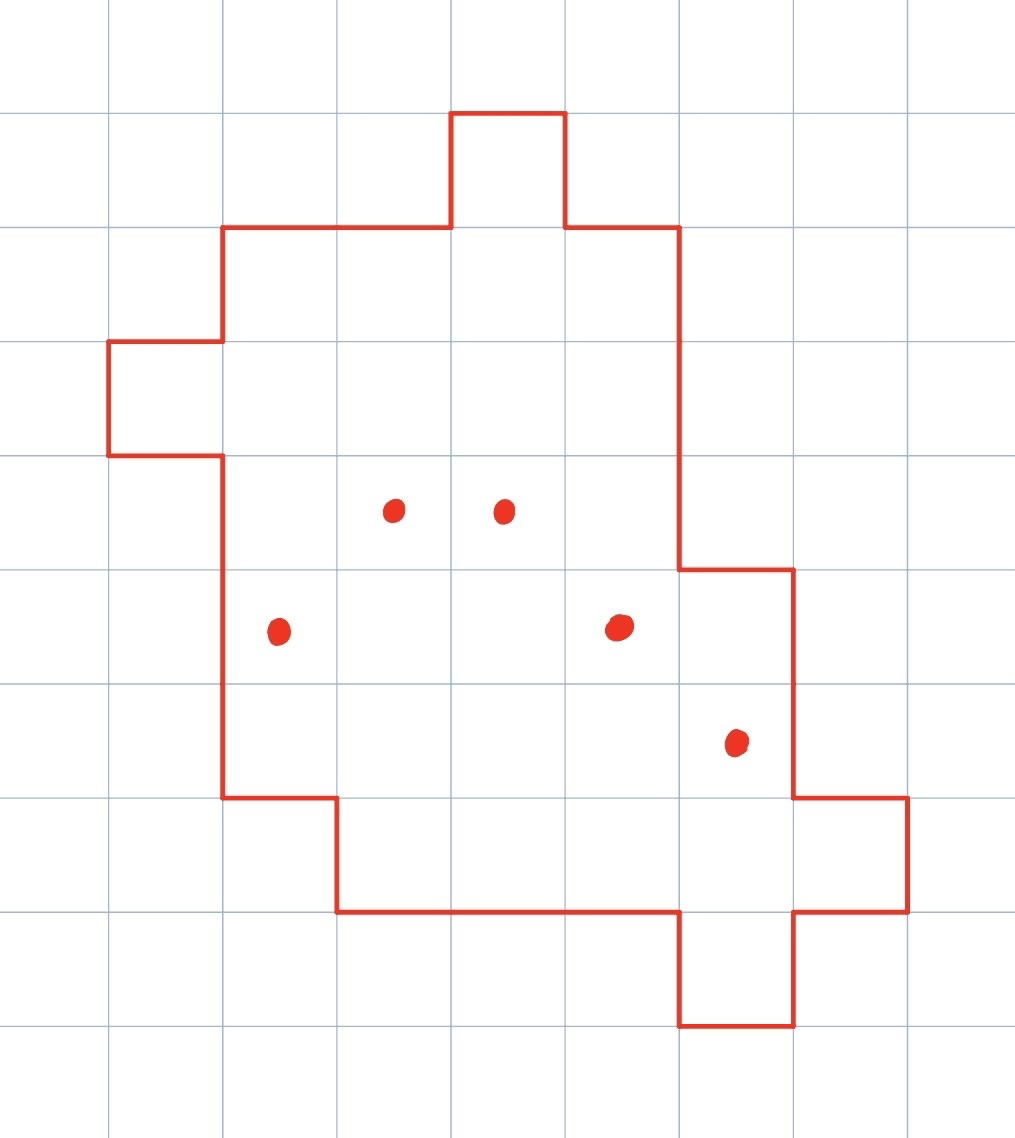
\includegraphics[width=0.2\linewidth]{ЭлМШ 2023-2024/VIII блок/Шиншиллы/HW_Cutting_2.png}
\end{figure}

\problem{3}
Разделите фигуру на 48 равных частей так, чтобы линия разреза шла по сторонам квадратов и сложите из них квадрат.
\begin{figure}[h]
        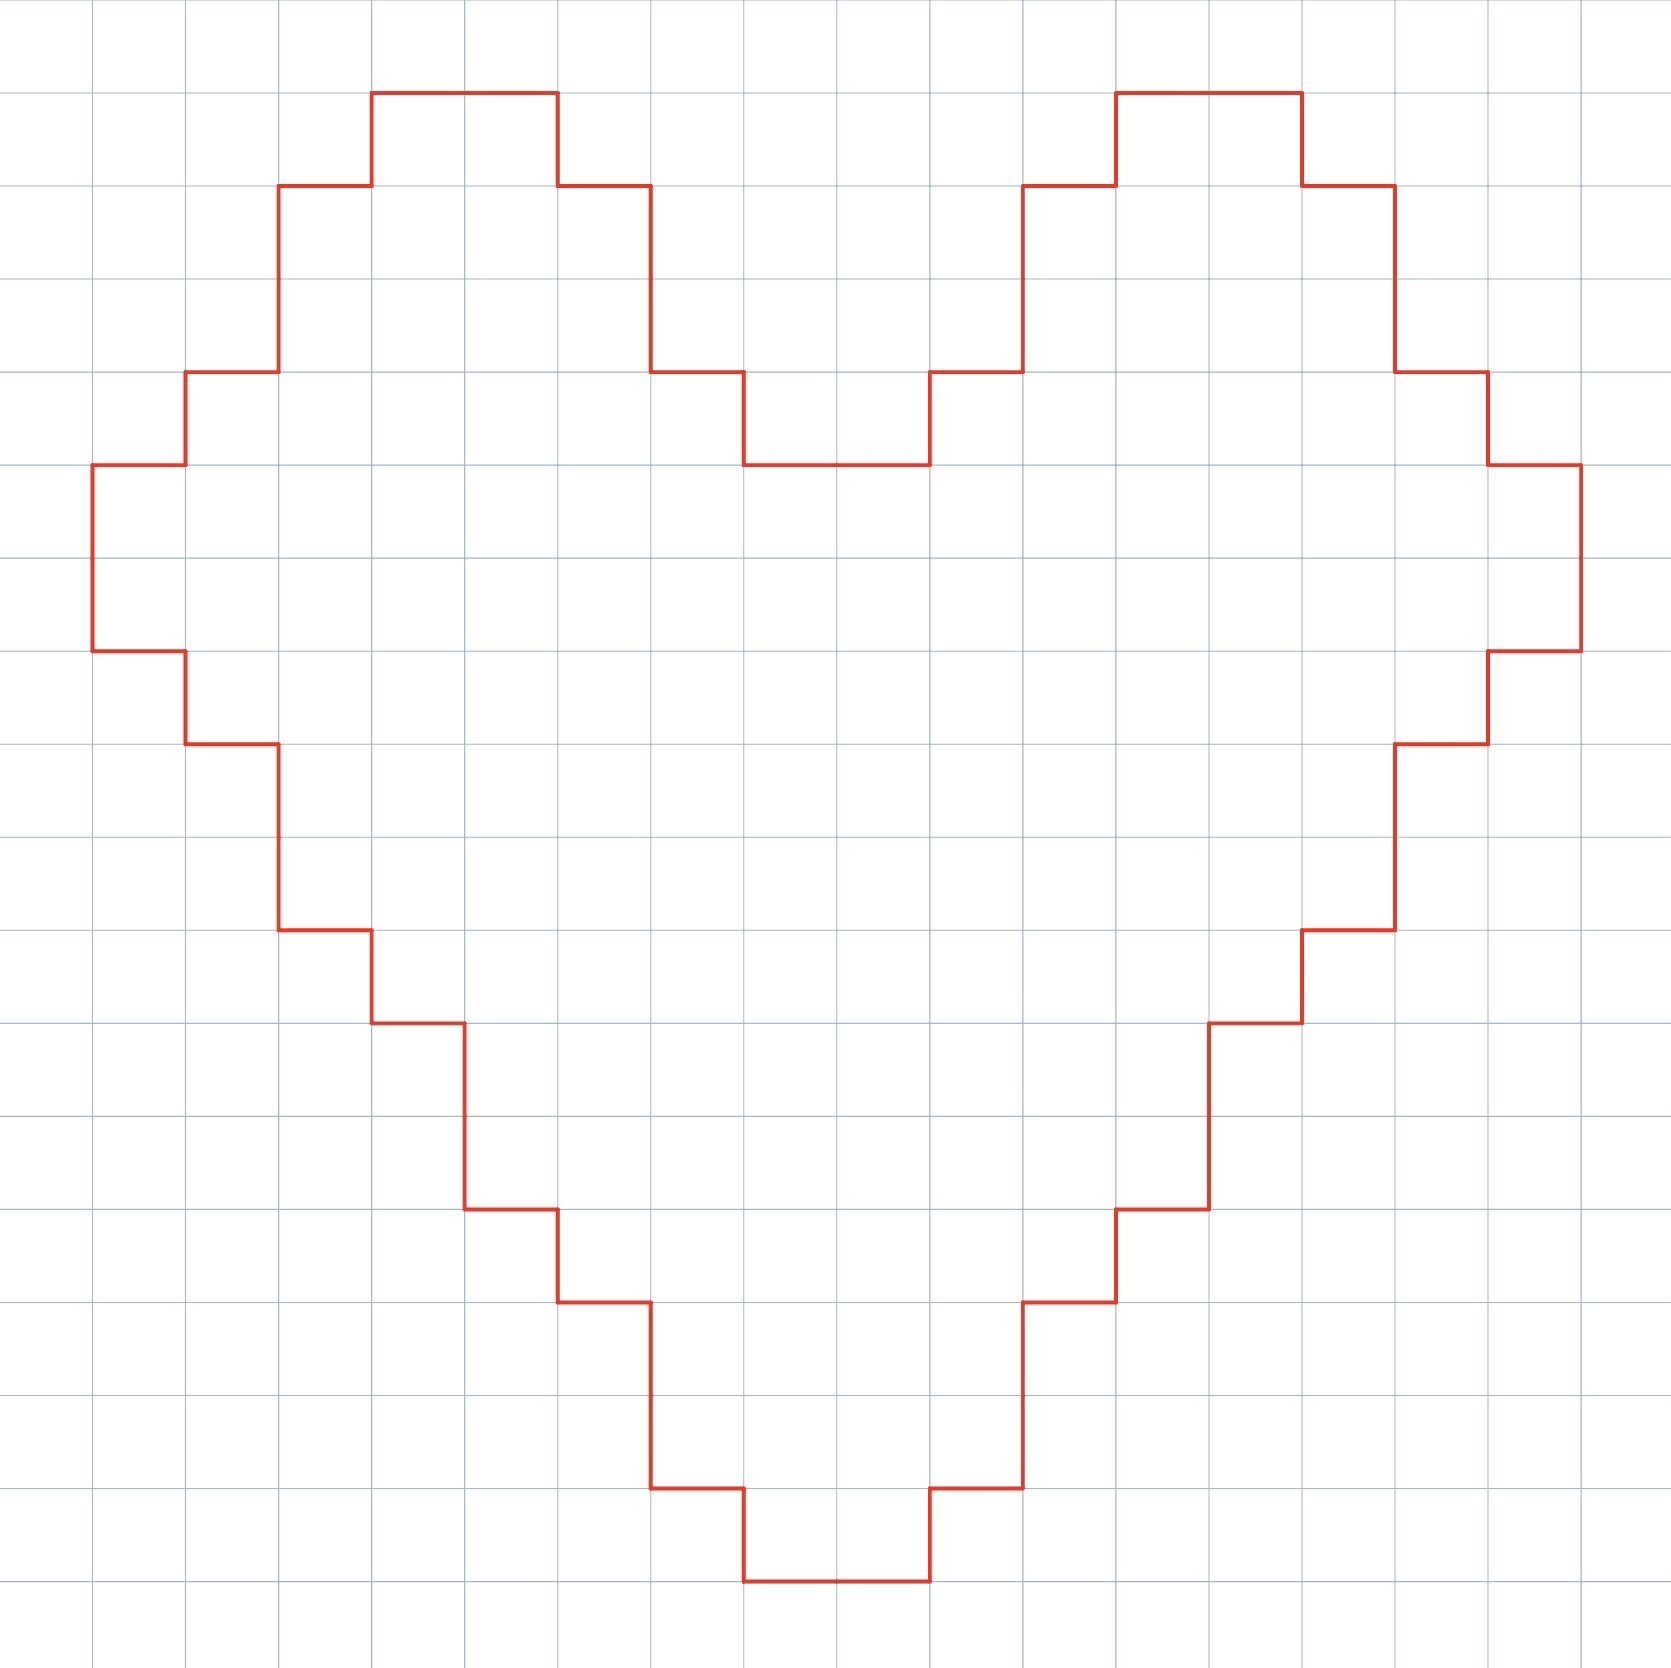
\includegraphics[width=0.2\linewidth]{ЭлМШ 2023-2024/VIII блок/Шиншиллы/HW_Cutting_3.png}
\end{figure}

\newpage

\hspace{3mm}

\problem{4}
Разрежьте фигуру на четыре равные части по линиям сетки, причем в каждой из частей должно быть по две точки.
\begin{figure}[h]
        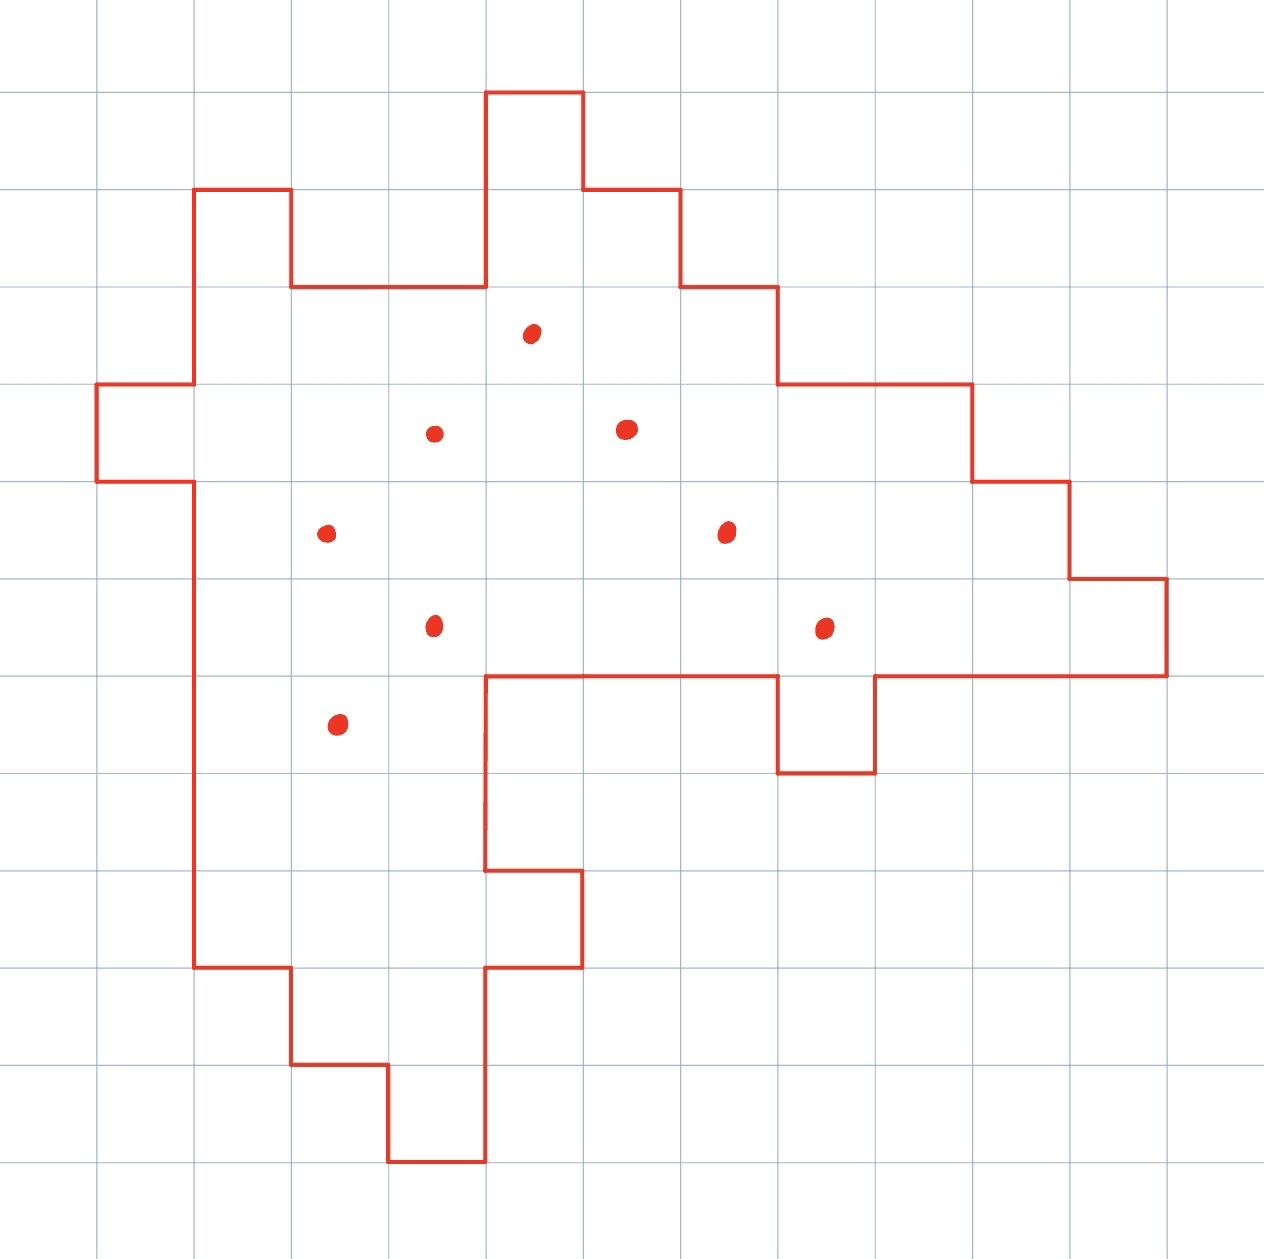
\includegraphics[width=0.2\linewidth]{ЭлМШ 2023-2024/VIII блок/Шиншиллы/HW_Cutting_4.png}
\end{figure}